\documentclass[final]{beamer}
\usepackage{grffile}
\usepackage{graphbox}
\mode<presentation>{\usetheme{I6pd2}}
\usepackage[english]{babel}
\boldmath
\usepackage[orientation=landscape,size=a1,scale=1.24,debug]{beamerposter}

\usepackage{snapshot} % will write a .dep file with all dependencies, allows for easy bundling
\usepackage{caption}
\usepackage{bibentry}
\usepackage{array,booktabs,tabularx}
\usepackage{qrcode}
\newcolumntype{Z}{>{\centering\arraybackslash}X} % centered tabularx columns
\newcommand{\pphantom}{\textcolor{ta3aluminium}} % phantom introduces a vertical space in p formatted table columns??!!
\captionsetup{labelformat=empty}
\listfiles

%%%%%%%%%%%%%%%%%%%%%%%%%%%%%%%%%%%%%%%%%%%%%%%%%%%%%%%%%%%%%%%%%%%%%%%%%%%%%%%%%%%%%%
\graphicspath{{figures/}}
 
\title{Genomics on the frontline of infectious disease outbreak response and animal health emergency investigations at the Canadian Food Inspection Agency}
\author{
Oliver Lung,
Peter Kruczkiewicz,
Oksana Vernygora,
Josip Rudar,
Katherine Handel,
Mathew Fisher,
Daniel Sullivan,
Michelle Nebroski,
Asma Sultana,
Hai Hoang Nguyen,
and Justin Hawkins
}
\institute{
Canadian Food Inspection Agency, National Centre for Foreign Animal Disease, Winnipeg, Canada
}

%%%%%%%%%%%%%%%%%%%%%%%%%%%%%%%%%%%%%%%%%%%%%%%%%%%%%%%%%%%%%%%%%%%%%%%%%%%%%%%%%%%%%%
\newlength{\columnheight}
\setlength{\columnheight}{104cm}


%%%%%%%%%%%%%%%%%%%%%%%%%%%%%%%%%%%%%%%%%%%%%%%%%%%%%%%%%%%%%%%%%%%%%%%%%%%%%%%%%%%%%%
\begin{document}
\begin{frame}
\begin{columns}
  \begin{column}{.5\textwidth}
  \begin{beamercolorbox}[center,wd=\textwidth]{postercolumn}
  \begin{minipage}[T]{.95\textwidth}  % tweaks the width, makes a new \textwidth
  \parbox[t][\columnheight]{\textwidth}{ % must be some better way to set the the height, width and textwidth simultaneously
  % Since all columns are the same length, it is all nice and tidy.  You have to get the height empirically
  % ---------------------------------------------------------%
  % fill each column with content            
  \begin{block}{Introduction}
    \vskip1.5ex
    \begin{columns}
      \begin{column}{0.62\textwidth}
        The Canadian Food Inspection Agency (CFIA) National Centre for Foreign Animal Disease (NCFAD) Genomics Unit provides genomics and bioinformatics support for outbreaks, diagnostics, surveillance, and research on known, novel, and unexpected infectious diseases in animals nationally and internationally. 
        In addition to containment level (CL) 2 sequencing capabilities, NCFAD’s Genomics Unit operates a unique CL 3 sequencing facility, allowing for convenient sequencing of samples from CL 3, 3+ and 4 laboratories.  Its use of both short-read Illumina and long-read Oxford Nanopore sequencing technologies, along with automation in both the wet- and dry-lab, has allowed it to build the capability and capacity to sequence, analyze, and accurately characterize large volumes of diverse samples. The NCFAD’s Genomics Unit supports and participates in collaborative projects with a wide range of government and NGO partners.
      \end{column}
      \begin{column}{0.35\textwidth}
        \includegraphics[width=\linewidth]{images/intro-images-tiled.png}
      \end{column}
    \end{columns}
  \end{block}

  \begin{block}{Overview of the NCFAD Genomics Unit}
    We have structured our operations to maximize efficiency and reproducibility through automation and deployment of systems for genomics data and information management, analysis and reporting to better support scientific research and response to animal health emergencies such as the ongoing H5N1 avian influenza outbreak.
      
    \includegraphics[width=1.0\linewidth]{images/2024-05-07-ncfad-genomics-unit-workflow-sample-to-results.pdf}
  \end{block}
            
  \vskip-1ex
  \begin{block}{Rapid Influenza Sequencing and Analysis Using Nanopore and nf-flu}
    % \vskip1.5ex
    \begin{columns}
      \begin{column}{0.4\textwidth}
        \vskip-2ex

        In response to the 2021 H5N1 Influenza A virus (IAV) outbreak, we developed an end-to-end workflow for sequencing and analysis providing comprehensive results within hours of sample receipt. Oxford Nanopore GridION sequencing and nf-flu Nextflow pipeline analysis have allowed us to rapidly and cost effectively sequence and analyse over 5,200 IAV sequenced between December 2021 and April 2024.

        \vskip1.0em

        \begin{itemize}
          \item \textbf{Sequencer:} ONT GridION
          \item \textbf{Protocol:} PCR \& Rapid Barcoding
          \item \textbf{Pipeline:} nf-flu Nextflow pipeline
        \end{itemize}

      \end{column}
      \begin{column}{0.58\textwidth}
        \vskip1.5ex
        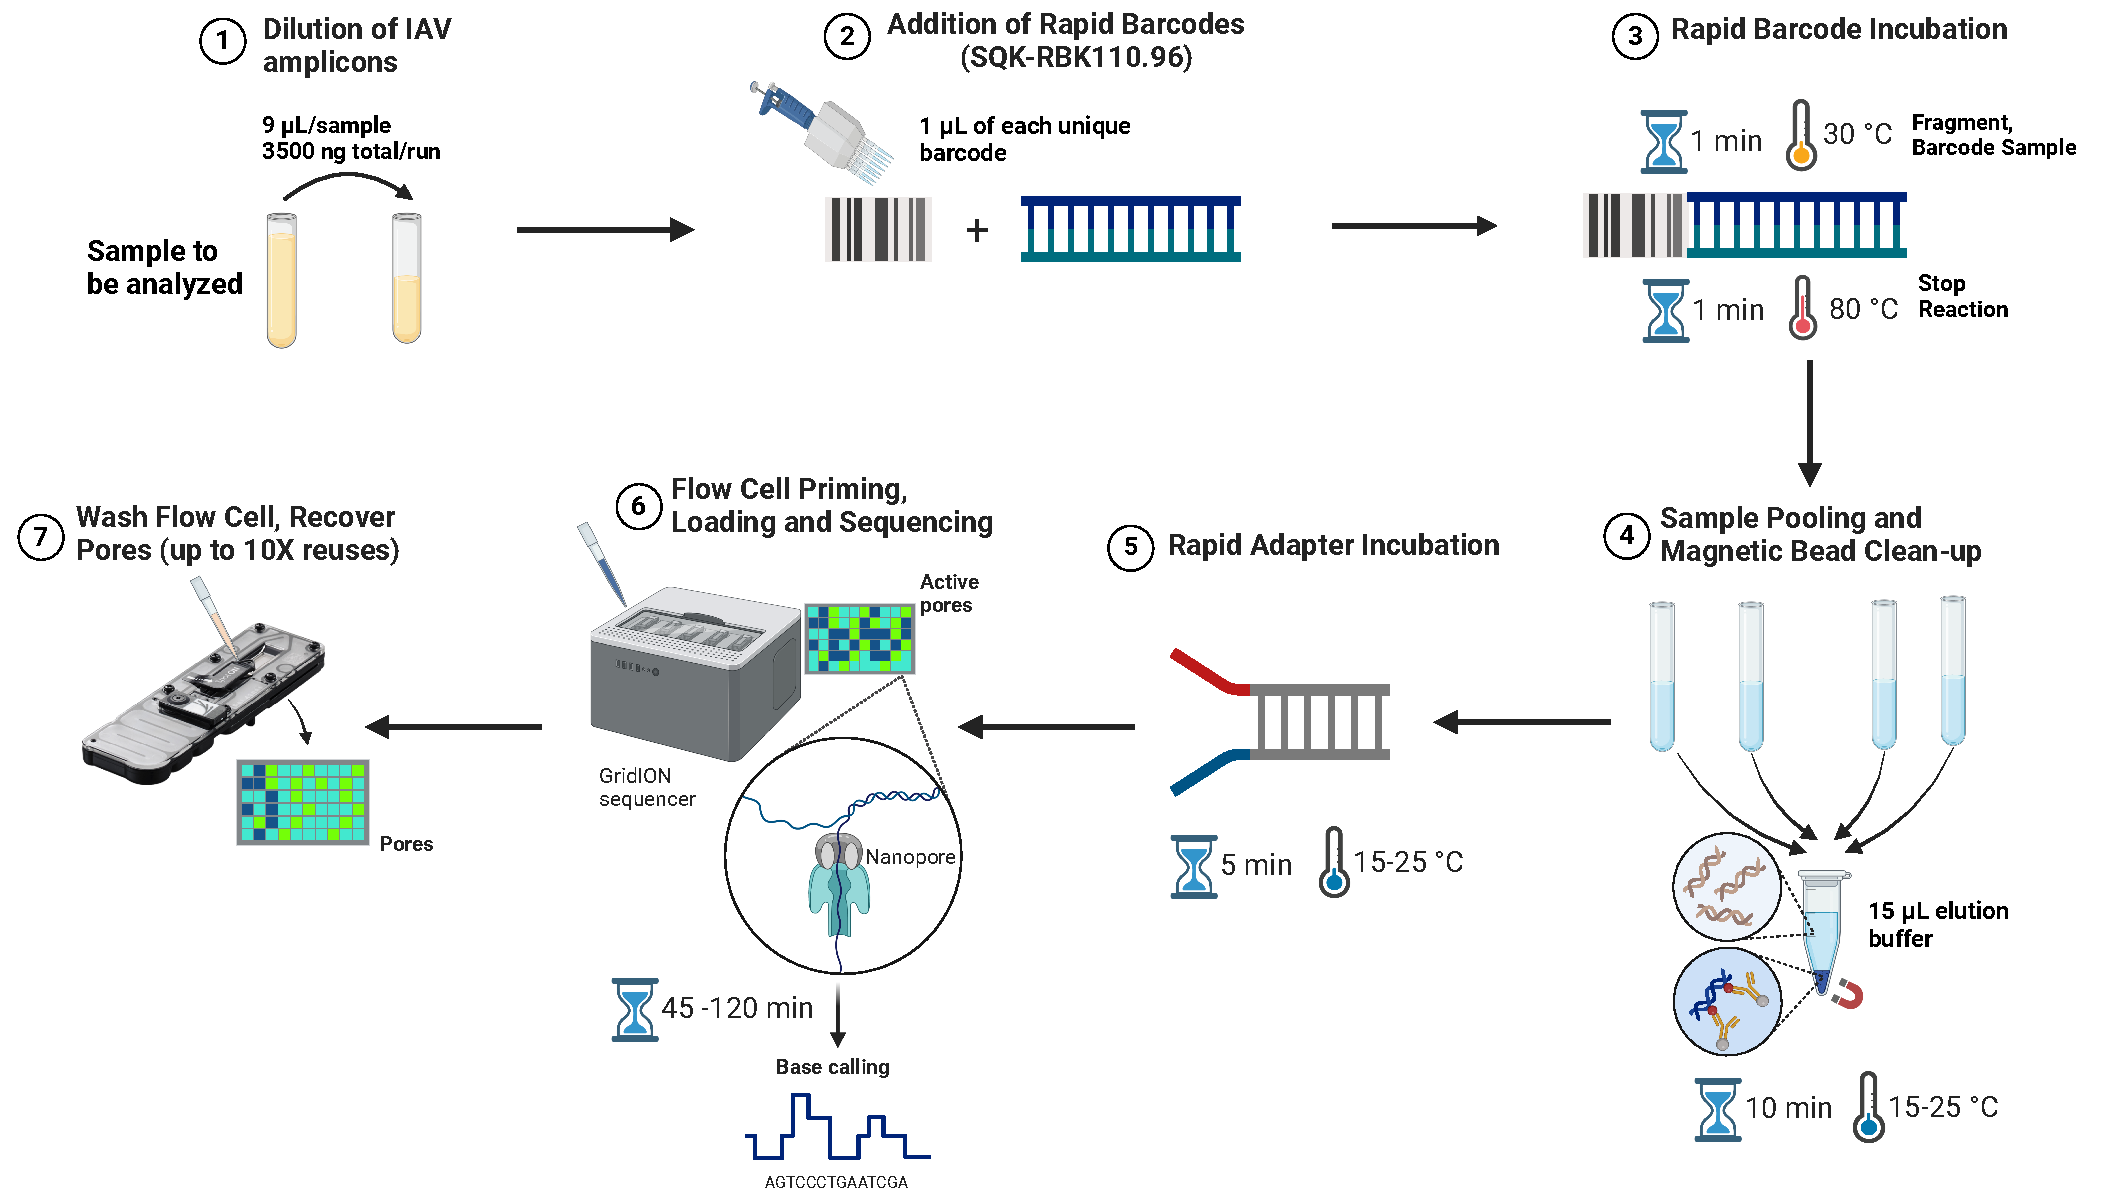
\includegraphics[width=1.0\linewidth]{images/AIV Nanopore Sequencing Protocol-1.pdf}
      \end{column}
    \end{columns}
  \end{block}
  }
  \end{minipage}
  \end{beamercolorbox}
  \end{column}
  % ---------------------------------------------------------%
  % end the column


      % ---------------------------------------------------------%
  % Set up a column 
  \begin{column}{.5\textwidth}
  \begin{beamercolorbox}[center,wd=\textwidth]{postercolumn}
  \begin{minipage}[T]{.95\textwidth} % tweaks the width, makes a new \textwidth
  \parbox[t][\columnheight]{\textwidth}{ % must be some better way to set the the height, width and textwidth simultaneously
  % Since all columns are the same length, it is all nice and tidy.  You have to get the height empirically
  % ---------------------------------------------------------%
  % fill each column with content
  \begin{block}{Automating Bioinformatics Analyses With Nextflow}
    \vskip1.5ex
    \begin{columns}
      \begin{column}{0.29\textwidth}
        The nf-flu Nextflow pipeline is an example of the bioinformatics tools and pipelines that the NCFAD has developed.
        These pipelines are routinely used at the NCFAD for analysis of viral sequencing data including from the ongoing H5N1 IAV outbreak.

        Tools and pipelines available at github.com/CFIA-NCFAD.
      \end{column}
      \begin{column}{0.69\textwidth}
        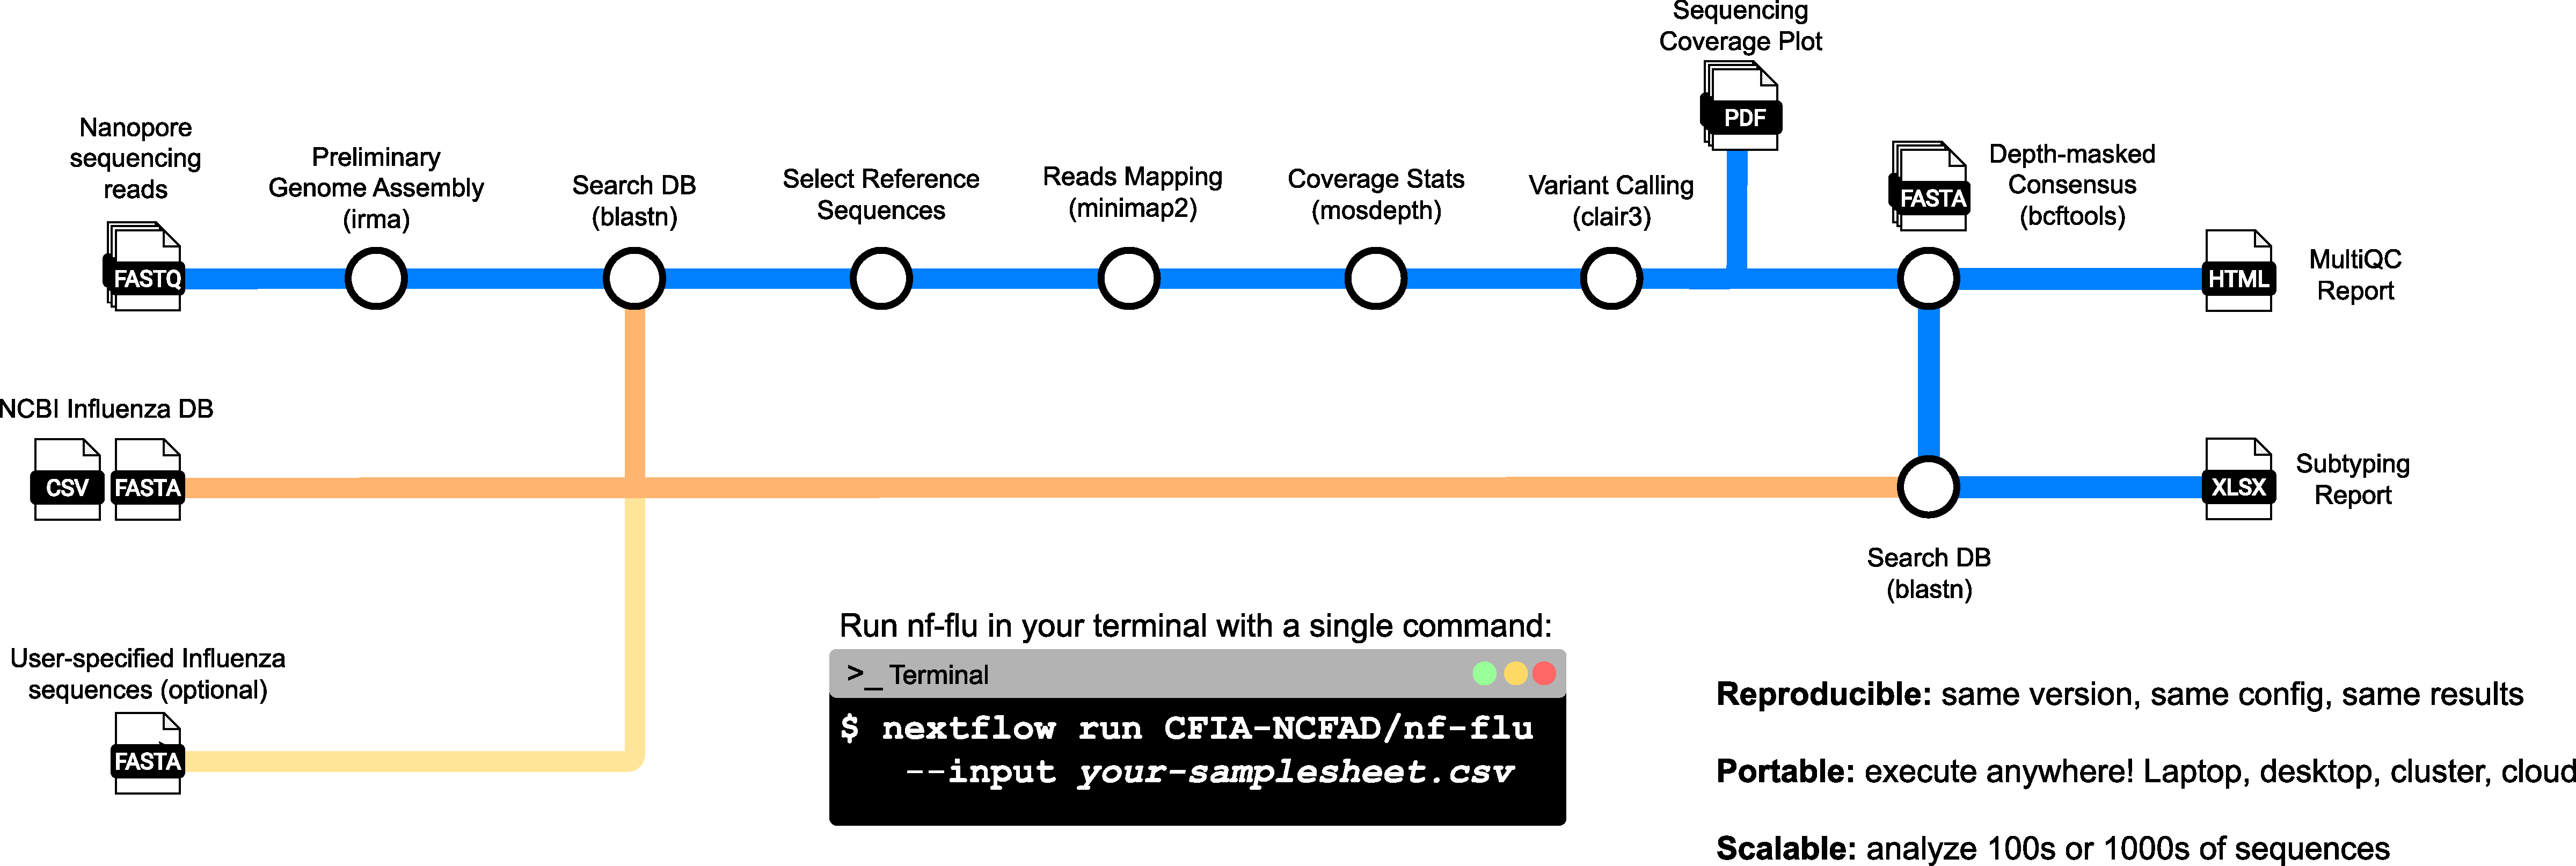
\includegraphics[width=1.0\linewidth]{images/nf-flu-workflow-diagram.pdf}
      \end{column}
    \end{columns}
  \end{block}

  % \vskip-1ex
  \begin{block}{Virus Sequencing and Novel Virus Discovery}
    % \vskip0.0ex
    \begin{columns}
    \begin{column}{.26\textwidth}
      \parbox[t]{\textwidth}{
      \begin{table}
      \caption{Viruses identified in samples sequenced from 2017 to April 30, 2024.}
      \begin{tabular}{l r}
      \textbf{Virus} & \textbf{Count} \\
      Influenza A & 8,345 \\
      SARS-CoV-2 & 831 \\
      Foot-and-mouth-disease & 552 \\
      Vesicular stomatitis & 247 \\
      Classical swine fever & 227 \\
      Senecavirus A & 171 \\
      Rabbit hemorrhagic disease & 141 \\
      African swine fever & 133 \\
      \emph{Others} & 3,031 \\
      \end{tabular}
      
      \end{table}
      }
    \end{column}
    \begin{column}{.01\textwidth}
    % empty spacer column
    \end{column}
    \begin{column}{.67\textwidth}
    \begin{tabular}{c l c}
      & \textbf{Novel Virus Publication Title} & \textbf{Link} \\
      % Senecavirus cetus
      \vtop{\null\hbox{
      
\includegraphics[height=20pt]{images/cetacean.pdf}
      }}
      &
      \vtop{\null\hbox{
      \parbox[t]{.8\textwidth}{
      \emph{\textbf{Senecavirus cetus}} a novel picornavirus isolated from cetaceans represents a major host switching to the marine environment
      }}}
      &
      \vtop{\null\hbox{
      \qrcode[height=40pt]{https://doi.org/10.21203/rs.3.rs-3900733/v1} 
      }}
      \\
      % Mutorquevirus
      \vtop{\null\hbox{
      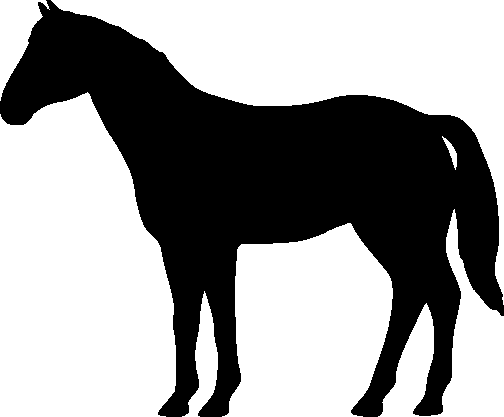
\includegraphics[height=40pt]{images/horse.pdf}
      }}
      &
      \vtop{\null\hbox{
      \parbox[t]{.8\textwidth}{
      Discovery and comparative genomic analysis of a novel equine anellovirus,
      representing the first complete \textbf{Mutorquevirus} genome
      }}}
      &
      \vtop{\null\hbox{
      \qrcode[height=40pt]{https://www.nature.com/articles/s41598-023-30875-7} 
      }}
      \\
      % Elk circovirus
      \vtop{\null\hbox{
      
\includegraphics[height=40pt]{images/elk.pdf}
      }}
      & 
      \vtop{\null\hbox{
      \parbox[t]{.8\textwidth}{
      Discovery and comparative genomic analysis of \textbf{elk circovirus (ElkCV)}, 
      a novel circovirus species and the first reported from a cervid host
      }}}
      & 
      \vtop{\null\hbox{
      \qrcode[height=40pt]{https://www.nature.com/articles/s41598-020-75577-6} 
      }}
      \\
      % Goose coronavirus
      \vtop{\null\hbox{
      
\includegraphics[height=40pt]{images/goose.pdf}
      }}
      & 
      \vtop{\null\hbox{
      \parbox[t]{.8\textwidth}{
      Genome organization of Canada \textbf{goose coronavirus CB19},
      a novel species identified in a mass die-off of Canada Geese 
      }}}
      & 
      \vtop{\null\hbox{
      \qrcode[height=40pt]{https://www.nature.com/articles/s41598-019-42355-y}
      }}
      \\
    \end{tabular}
    \end{column}
    \end{columns}
  \end{block}

  % \vskip-1ex
  \begin{block}{Other Activities of the NCFAD Genomics Unit}
    \begin{columns}
      \begin{column}{0.7\textwidth}
        \begin{itemize}
          \item Genomics and bioinformatics support for WOAH and FAO Reference Laboratories such as
          \begin{itemize}
            \item Influenza A virus (IAV) from Ghana; foot-and-mouth disease virus (FMDV) from Brazil and Nigeria; classical swine fever virus (CSFV) from Colombia; African swine fever virus (ASFV) from Viet Nam and Nigeria; rabbit hemorrhagic disease virus (RHDV) from Ghana; bovine viral diarrhea virus (BVDV)
          \end{itemize}
          \item Investigate infectious disease and mortality events in
          \begin{itemize}
            \item farmed animals (mink, elk, cattle, pigs), terrestrial wildlife (muskoxen, caribou, black-tailed deer) and marine wildlife (great white shark, Stellar sea lions, Pacific walrus, sea lion)
          \end{itemize}
          \item Viruses in wild-life and disease vectors
          \item Machine learning \& AI for biomarker discovery and sequence analysis
          \item Regular Canadian and international wet- and dry-lab exercises
          \begin{itemize}
            \item Annual UNSGM dry-lab external quality assurance exercises (2021-2024)
            \item Microbial Investigation Process Inter-Laboratory Exchange (MIPIE) (2020-2022)
            \item Agnostic Metagenomics for Identification of Novel or Synthetically Modified Microorganisms (2024)
          \end{itemize}
        \end{itemize}
      \end{column}
      \begin{column}{0.3\textwidth}
        \begin{figure}
          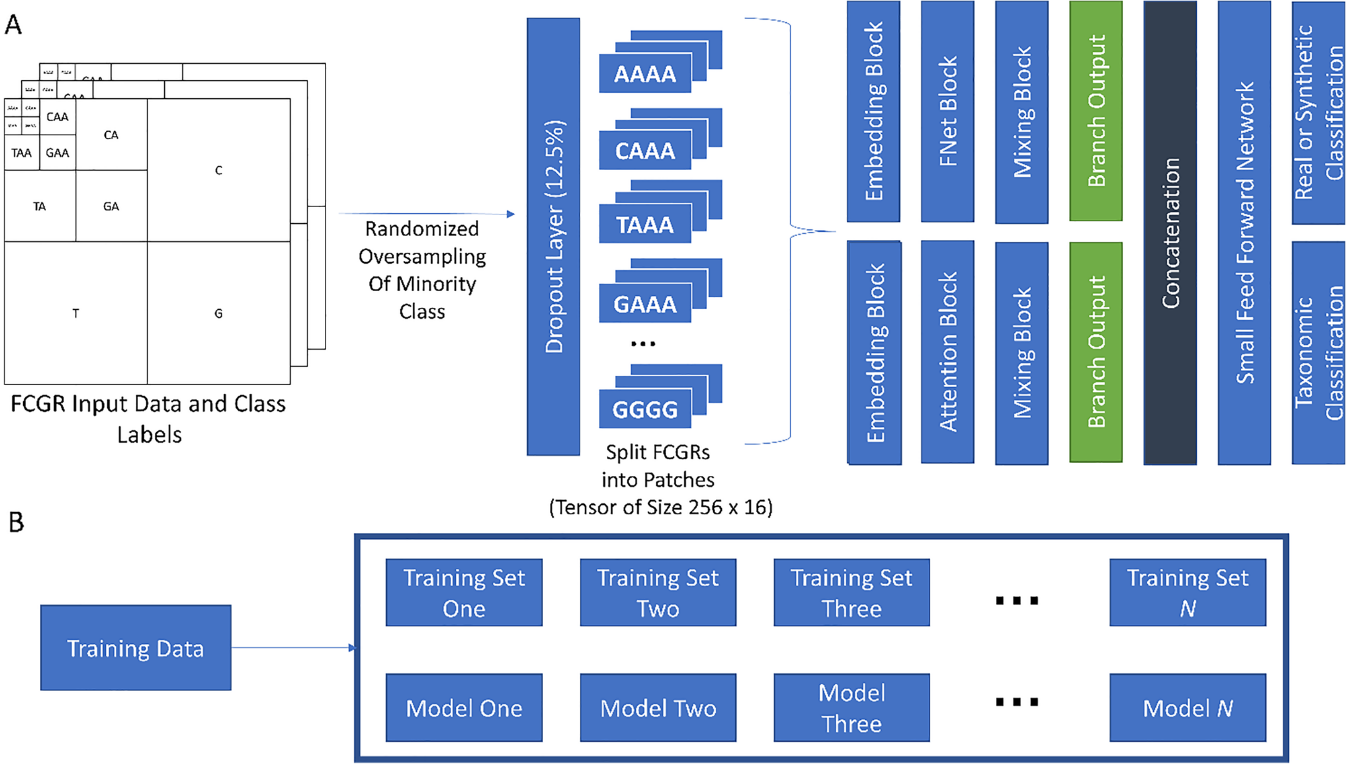
\includegraphics[width=0.95\linewidth]{images/neural-net-culicidae-mitogenomes-figure-4.png}
          \caption{\tiny Deep neural network architecture for identification of mosquito classification from Harrison et al (2022) (doi: 10.1038/s41598-022-26236-5)}
        \end{figure}
        

        \begin{figure}
          
        \centering
        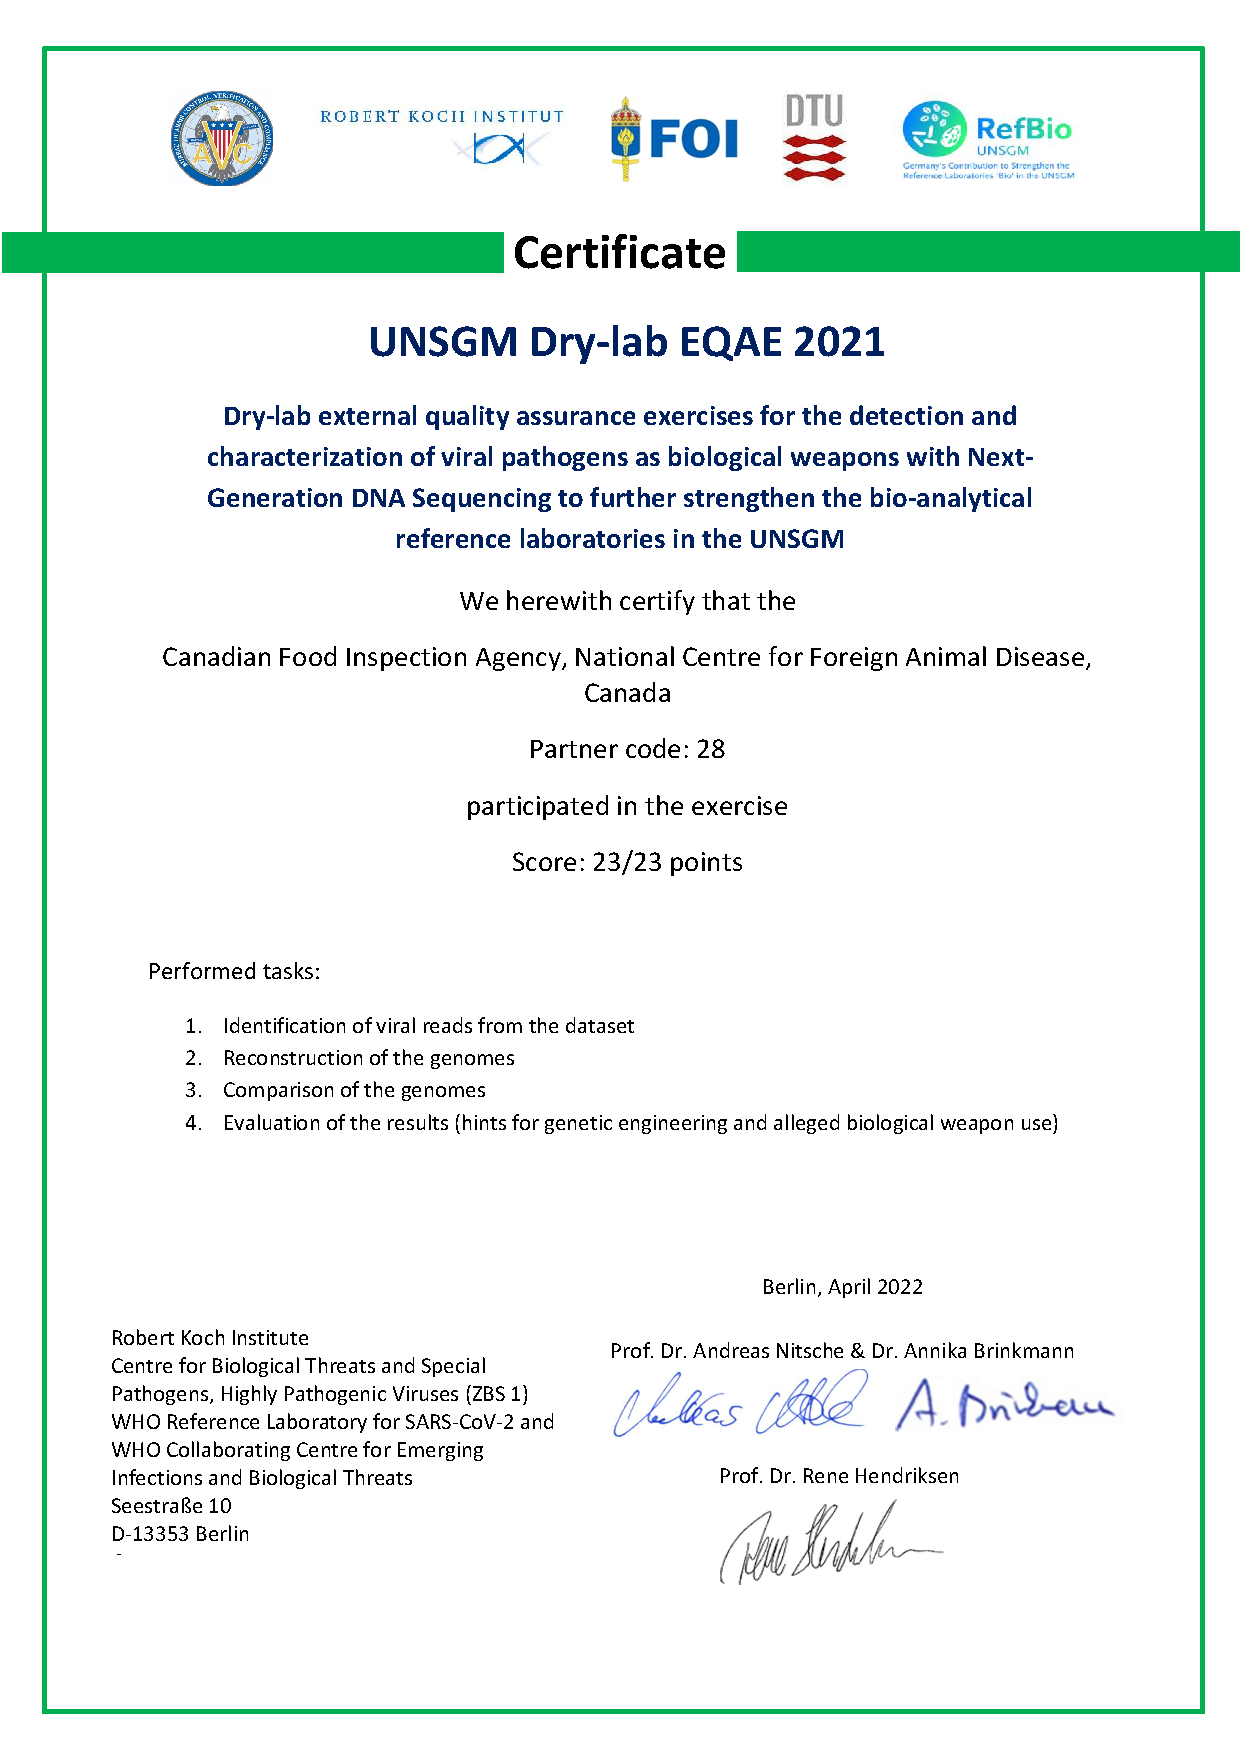
\includegraphics[align=c,width=0.4\linewidth]{images/UNSGM_DryLab_Certificate-28.pdf}
        
\includegraphics[align=c,width=0.3\linewidth]{images/IWTSDLogo.png}
        
        \end{figure}
        
      \end{column}
    \end{columns}
  \end{block}

  % \vskip-1ex
  \begin{block}{Acknowledgements}
    % \footnotesize
    Financial support was provided by the CFIA, Canadian Safety and Security Program (CSSP), LabsCanada, Genomics Research and Development Initiative (GRDI).
  \end{block}
  % \vskip-1ex
  % incomplete list of affiliations
  % \begin{block}{Affiliations}
  %   \scriptsize
  %   Agriculture and Agri-Food Canada;
  %   Alaska Veterinary Pathology Services;
  %   Atlantic Veterinary College;
  %   BC Animal Health Centre;
  %   Canadian Wildlife Health Cooperative;
  %   Dalhousie University;
  %   Environment and Climate Change Canada;
  %   Fisheries and Oceans Canada;
  %   Ontario Ministry of Natural Resources and Forestry;
  %   Public Health Agency of Canada;
  %   Sunnybrook Research Institute;
  %   University of Alaska Anchorage;
  %   University of Calgary;
  %   University of Guelph;
  %   University of Manitoba;
  %   University of Prince Edward Island;
  %   University of Texas Medical Branch
  % \end{block}

  }
  % ---------------------------------------------------------%
  % end the column
  \end{minipage}
  \end{beamercolorbox}
  \end{column}
  % ---------------------------------------------------------%
  % end the column
\end{columns}
\vskip1ex
%\tiny\hfill\textcolor{ta2gray}{Created with \LaTeX \texttt{beamerposter}  \url{http://www-i6.informatik.rwth-aachen.de/~dreuw/latexbeamerposter.php}}
\tiny\hfill{Created with \LaTeX \texttt{beamerposter}  \url{http://www-i6.informatik.rwth-aachen.de/~dreuw/latexbeamerposter.php} \hskip1em}
\end{frame}
\end{document}


%%%%%%%%%%%%%%%%%%%%%%%%%%%%%%%%%%%%%%%%%%%%%%%%%%%%%%%%%%%%%%%%%%%%%%%%%%%%%%%%%%%%%%%%%%%%%%%%%%%%
%%% Local Variables: 
%%% mode: latex
%%% TeX-PDF-mode: t
%%% End: